\documentclass[a4paper, 12pt]{article}
\usepackage{amssymb}
\usepackage{amsmath}
\usepackage{verbatim}
\setcounter{tocdepth}{3}
\usepackage{graphicx}
\usepackage{afterpage}
\usepackage{floatpag}
\usepackage{setspace}
\floatpagestyle{empty}
%\usepackage[a4paper, total={4in, 6in},margin=4in]{geometry}
\usepackage[export]{adjustbox}
%\usepackage[paperwidth=7.0in, paperheight=10.7in]{geometry}
%\usepackage{layout}
%\layout{layoutwidth=180mm,layoutheight=227mm}
%\geometry{a4paper,left=25mm,right=25mm,top=25mm,bottom=25mm,heightrounded}
%\usepackage[a4paper]{geometry}
\usepackage{listings}
\usepackage{subfigure}
\usepackage{wrapfig}
\usepackage[hyperindex=false,colorlinks=false]{hyperref}
\usepackage{fullpage}
\usepackage{tikz}
\usetikzlibrary{shapes.geometric, arrows}
\DeclareMathSizes{20}{20}{20}{20}

\tikzstyle{startstop}=[rectangle, rounded corners, minimum width=3cm, minimum height=1cm, text centered, text width=4cm, draw=black,fill=red!30]

\tikzstyle{io}=[trapezium, trapezium left angle=70, trapezium right angle=110, minimum width=3cm, minimum height=1cm, text centered, text width=4cm, draw=black, fill=blue!30]

\tikzstyle{process}=[rectangle, minimum width=3cm, minimum height=1cm, text centered, text width=4cm, draw=black,fill=orange!30]

\tikzstyle{decision}=[diamond, minimum width=3cm, minimum height=1cm, text centered, text width=4cm, draw=black, fill=green!30]

\tikzstyle{arrow}=[thick,->,>=stealth]

\begin{document}

\begin{titlepage}

%\newcommand{\HRule}{\rule{\linewidth}{0.5mm}} % Defines a new command for the horizontal lines, change thickness here
\newcommand{\HRule}{\rule{155mm}{0.5mm}} % Defines a new command for the horizontal lines, change thickness here

\center % Center everything on the page

%----------------------------------------------------------------------------------------
%   HEADING SECTIONS
%----------------------------------------------------------------------------------------

\textsc{\LARGE Technische Universit{\"a}t M{\"u}nchen}\\[1.5cm] % Name of your university/college
\textsc{\Large Chair For Computer Technology and Computer Organisation}\\[0.5cm] % Major heading such as course name

%----------------------------------------------------------------------------------------
%   TITLE SECTION
%----------------------------------------------------------------------------------------
\vspace{30mm}
\begin{center}
\Large\textit{Guided Research}
\end{center}
\HRule \\[0.4cm]
{ \Large \bfseries A Protocol for the Integration of Invasive Resource Management into Standard Batch Schedulers}\\[0.5cm] % Title of your document
\HRule \\[1.5cm]

%----------------------------------------------------------------------------------------
%   AUTHOR SECTION
%----------------------------------------------------------------------------------------
\vspace{48mm}
\begin{minipage}{0.4\textwidth}
\begin{flushleft} \large
\emph{Student:}\\
Nishanth Nagendra % Your name
\end{flushleft}
\end{minipage}
\begin{minipage}{0.4\textwidth} 
\begin{flushright} \large
\emph{Supervisor:} \\
Prof. Dr. Michael Gerndt \\~\\ % Supervisor's Name
\emph{Advisor:} \\
M.Sc. Isaias Alberto Compres Urena  % Advisor's Name
\end{flushright}
\end{minipage}\\[2cm]

% If you don't want a supervisor, uncomment the two lines below and remove the section above
%\Large \emph{Author:}\\
%John \textsc{Smith}\\[3cm] % Your name

%----------------------------------------------------------------------------------------
%   DATE SECTION
%----------------------------------------------------------------------------------------

{\large \today}\\[2cm] % Date, change the \today to a set date if you want to be precise

\end{titlepage}

\begin{center}
\huge \bfseries Acknowledgement
\end{center}
\thispagestyle{empty}
\vspace{35mm}
I would like to thank  Isaias for his constant support and guidance throughout the guided research especially when I faced some challenges in understanding certain topics. I would also like to thank Prof. Dr. Michael Gerndt for providing me with this opportunity to work on such an interesting topic.

\newpage

\begin{center}
\huge \bfseries Abstract
\end{center}
\thispagestyle{empty}
\vspace{35mm}

Invasive computing is a novel paradigm for the design and resource-aware programming of future parallel computing systems. It enables the programmer to write resource aware programs and the goal is to optimize the program for the available resources. Traditionally, parallel applications implemented using MPI are executed with a fixed number of MPI processes before submitting to a HPC(High Performance Computing) system. This results in a fixed allocation of resources for the job. Newer techniques in scientific computing such as AMR(Adaptive mesh refinement) result in applications exhibiting complex behavior where their resource requirements change during execution. Invasive MPI which is a part of an ongoing research effort to provide MPI extensions for the development of Invasive MPI applications will result in evolving jobs for the HPC systems at runtime supporting such AMR techniques. Unfortunately, using only static allocations result in the evolving applications being forced to execute using their maximum resource requirements that may lead to an inefficient resource utilisation. In order to support such parallel evolving applications at HPC centers there is an urgent need to investigate and implement extensions to existing resource management systems or develop an entirely new one. These supporting infrastructures must be able to handle these evolving jobs and also the legacy rigid jobs intelligently and hence newer protocols for integration of such invasive resource management into existing standard batch systems needs to be now explored.

\newpage
\thispagestyle{empty}
\tableofcontents
\newpage

\setcounter{page}{1}
\section{Introduction}
Invasive computing is a novel paradigm for the design and resource-aware programming of future parallel computing systems. It enables the programmer to write efficient resource aware programs. This approach can be used to allocate, execute on and free resources during execution of the program. HPC infrastructure like Clusters, Supercomputers execute a vast variety of jobs, majority of which are parallel applications. These centers use intelligent resource management systems that should not only perform tasks of job management, resource management and scheduling but also satisfy important metrics like higher system utilization, job throughput and responsiveness. Traditionally, MPI applications are executed with a fixed number of MPI processes but with Invasive MPI they can evolve dynamically at runtime in the number of their MPI processes. This in turn supports advanced techniques like AMR where the working set size of applications change at runtime. These advancements entail an immediate need for stronger and intelligent resource management systems that can provide efficient resource utilization at HPC centers. They should also now be able to achieve much higher system utilisation, energy efficiency etc. compared to their predecessors due to elasticity of the applications.\par
\noindent
\\Under the collaborative research project funded by the German research foundation(DFG) in the Transregional Collaborative Research Centre 89(TRR89), research efforts are being made to investigate Invasive computing approach vertically at different levels of abstraction right from the hardware up to the application level with all the intermediate levels. Invasive MPI is one such effort towards invasive programming with MPI where the application programmer has MPI extensions available using which he/she can specify at certain safe points in the program to allow for elasticity which means the application can evolve.

\subsection{Resource Management}
In order to support such parallel evolving applications at HPC centers there is an urgent need to investigate and implement extensions to existing resource management systems or develop an entirely new one. These supporting infrastructures must be able to handle the new kind of evolving jobs/applications and the legacy rigid jobs intelligently keeping in mind that they should now be able to achieve much higher system utilisation, energy efficiency etc compared to their predecessors due to the elasticity of the applications. Two of the most widely used resource managers on HPC systems are SLURM and TORQUE. The 2 major components in general of any sophisticated resource manager are the batch scheduler and the process manager.
\subsection{Batch Scheduling}
The batch scheduler accepts job descriptions given by end users some of which mention as to how long the job would run and the amount of resources it will need. It maintains a queue of jobs and dispatches them to the process manager based on some criteria and algorithms. The decisions made depend on the state of resources and also others like job priorities, fairness, waiting times etc. The process manager on the other hand has lesser intelligence and does the task of mapping the processes of a parallel application on the hardware based on the node list provided to it by the batch scheduler. In the context of invasive computing we need to be investigate for new requirements in the interaction between the batch scheduler and process manager. The decisions made by the batch scheduler need to be influenced to support evolving jobs.\par
\noindent
\\In contrast to the earlier uni-directional communication from batch scheduler to process manager, we now need to support a bi-directional communication between the two. The capabilities of existing batch schedulers could be leveraged rather than having to replace an entire system with a new one. The possiblity of supporting a new interface for the existing batch scheduler needs to be explored such that it communicates with a new invasive process management that controls a dedicated partition to support invasive computing. An investigation needs to be done on whether the existing interface of batch schedulers towards process manager could be extended or re-used and also on the possiblity of receiving feedback from the invasive process manager to allow the batch scheduler to be influenced. The invasive process manager one level below in the hierarchy as shown in the figure below will work on local metrics of the dedicated invasive partition within the cluster allocated by the batch scheduler. Whereas the batch scheduler will work on another set of metrics at the upper level for which it will want to optimize its decision making.\par
\noindent
\\The investigations of this guided research are an initial study that will support the continuing research effort for developing Invasive MPI and extended resource management systems to support Invasive computing systems.

\begin{figure}[h]
\centering
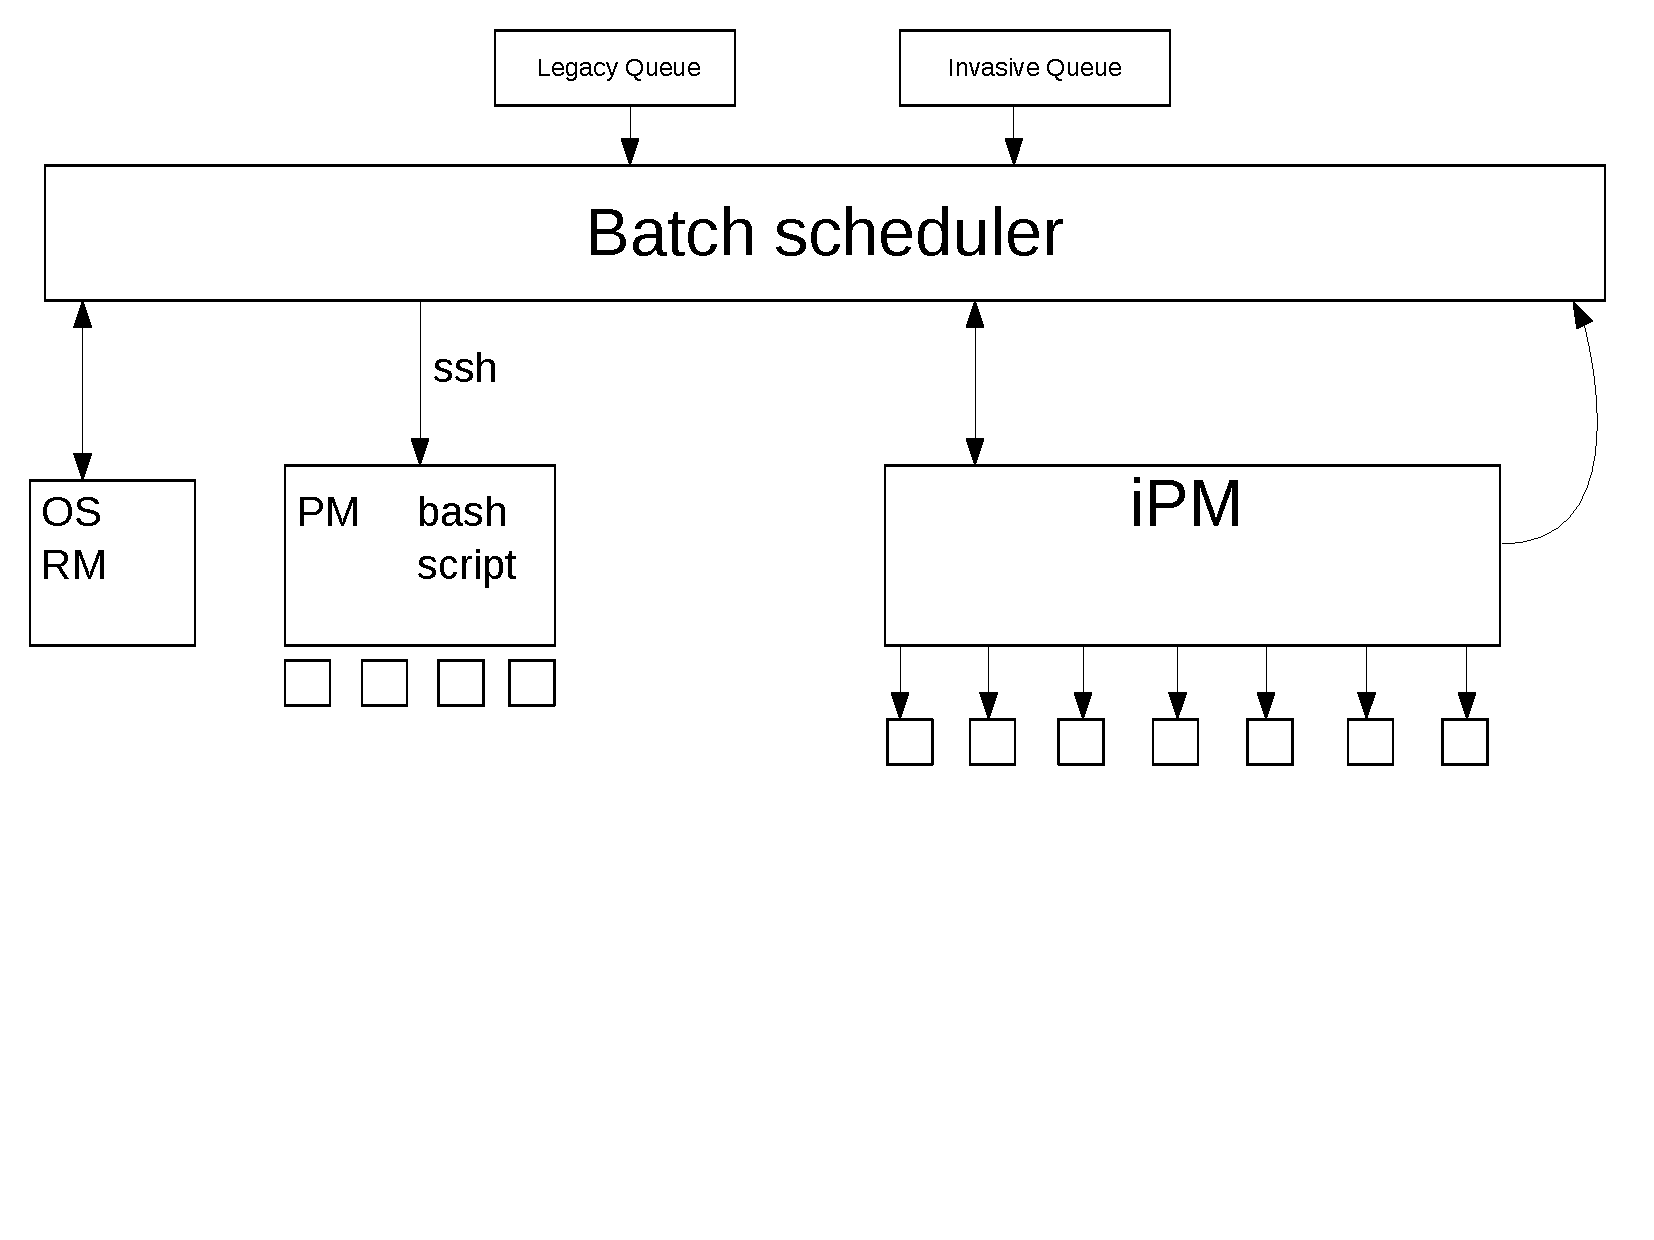
\includegraphics[width=0.65\textwidth, clip, trim=0mm 60mm 0mm 0mm]{data/architecture.pdf}
\vspace{-0.15in}
\caption{Invasive resource management architecture}
\label{fig:arch}
\end{figure}

\subsection{Software Requirements}
The project has been implemented in C with the help of an API(Linux version) provided by a commercial software suite for C++.\\~\\
\textbf{\boldmath$FICO^{TM}$ Xpress Optimization Suite:}   FICO Xpress Optimization Suite is a sophisticated mathematical modeling and optimization software. Its tools enable operational research and management professionals, analysts, and consultants to rapidly develop optimization applications that solve complex, real-world business and customer engagement challenges. It provides easy ways to create, deploy and utilize business optimization solutions based on scalable high-performance algorithms, a flexible modeling environment and rapid application and reporting capabilities.\\~\\
Optimization problems have to be solved computationally to good approximation and require the usage of sophisticated optimization 
softwares that can provide a library(API- Application programming interface) for the programmer to do the same. The programmer can use this to
 implement an application demonstrating the solving methods for DNDP. This is first done by modeling the DNDP in the form of a bilevel mixed 
integer linear program via the API provided by FICO Xpress BCL component and using its optimization modules to solve the nested optimization 
problem of TAP.\par                   
%\begin{figure}[h]
%\centering
%\includegraphics[width=0.65\textwidth, clip]{./Xpress.jpg}
%\vspace{-0.15in}
%\caption{Xpress product suite}
%\label{fig:1}
%\end{figure}
\noindent
\textbf{Libraries for embedding:}   An option available from this software for embedding mathematical models into large applications is by developing a model directly in a programming language with the help of a model builder library \textit{Xpresss-BCL}. BCL(Builder Component Library) allows a user to formulate models with objects(decision variables, constraints, index sets) similar to those of a dedicated modeling language. All libraries are available for C, C++, Java, C\#, and Visual Basic(VB). For this project we will be using the library for C++.\\ \par
\noindent
The Xpress-BCL Builder Component Library(BCL) provides an environment in which the Xpress user may readily formulate and solve linear, mixed integer and quadratic programming models. Using BCL’s extensive collection of functions, complicated models may be swiftly and simply constructed, preparing problems for optimization.\\ \par
\noindent
Model formulation using Xpress-BCL is constraint-oriented. Such constraints may be built up either coefficient-wise, incrementally adding 
linear or quadratic terms until the constraint is complete, or through use of arrays of variables, constructing the constraint through a 
scalar product of variable and coefficient arrays. The former method allows for easier modification of models once constructed, whilst the 
latter enables swifter construction of new constraints. To complement the model construction routines, BCL supports a number of functions which allow a completed model to be passed directly to the Xpress-Optimizer, solved by the optimizer, and solution information reported back 
directly from BCL.
\newpage
\section{Invasive Computing}
The throughput of supercomputers depends not only on efficient job scheduling but also on the type of jobs that form the workload. Malleable jobs are most favourable for a cluster as they can dynamically adapt to a changing allocation of resources. The batch system can expand or shrink a running malleable job to improve system utilization, throughput, and response times. In the past, however the rigid nature of commonly used programming models like MPI made writing malleable applications a daunting task, which is why it remains largely unrealized. This is now changing. To improve fault tolerance, load imbalance, and energy efficiency in emerging exascale systems more adaptive programming paradigms are being investigated. Although they may offer better support for malleability, current batch systems still lack management facilities for malleable jobs and are therefore incapable of leveraging their potential. In this guided research we propose an extension to the SLURM resource manager to support malleable jobs.
\subsection{Job Classification}
As defined by Feitelson and Rudolph [1], jobs can be classified into four categories based on their flexibility.
\begin{itemize}
\item Rigid job: This is the most common type which requires a fixed number of processors throughout its execution.
\item Moldable job: In this kind of job the resource set can be molded or modified by the batch system before starting the job (e.g. to effectively fit alongside other rigid jobs). Once started its resource set cannot be changed anymore.
\item Evolving job: These kind of jobs request for resource expansion or shrinkage during their execution. Applications that use multiscale analysis like Quadflow or Adaptive mesh refinement(AMR) exhibit this kind of behavior typically due to unexpected increases in computations or having reached hardware limits(e.g. memory) on a node. 
\item Malleable job: The expansion and shrinkage of resources are initiated by the batch system in contrast to the evolving jobs. The application adapts itself to the changing resource set.
\end{itemize}
The first two types fall into the category of what is called as the static allocation since the allocation of rigid and moldable jobs must be finalized before the job starts. Whereas, the last two types fall under the category of dynamic allocation since this property of expanding or shrinking evolving and malleable jobs(together termed adaptive jobs) happens at runtime.\par
\noindent
Malleable jobs hold a strong potential to obtain high system performance. Batch systems can substantially improve the system utilization, throughput and response times with efficient shrink/expand strategies for malleable jobs. Similarly, applications also profit when expanded with additional resources as this can increase application speedup and improve load balance across the job’s resource set. Enabling malleable jobs in cluster systems requires three major components: (i) a parallel runtime that is able to adapt to a changing resource set, (ii) a batch system with dynamic allocation facilities, and (iii) a communication mechanism between the two. Traditionally, all batch systems support only static allocations.\par
\noindent
However, to meet the needs of improved fault tolerance, load imbalance, and energy efficiency in emerging exascale systems, adaptive programming paradigms are foreseen to play a significant role. it is an urgent necessity for batch systems to support dynamic allocation facilities and manage a mix of job types in order to reduce resource wastage, increase throughput and address the ever increasing user demand for faster response times. This work advances the state of art in batch job management by extending the SLURM batch system to support Invasive resource management by first proposing a negotiation protocol to integrate such an Invasive RM component into existing batch systems.
In some cases the traffic pattern can be regulated by some central authority, as for example, a network used for the transportation of military supplies or for a railroad network. It is obvious that in this case, the problem which the central authority faces is to determine the traffic pattern which minimizes the total cost over the whole network.\\ \par
\noindent
On, the other hand a broad class of transportation networks can be described as user optimized. Here travel patterns are set up by individual users each choosing the cheapest way(in the light of other user's decisions) to arrive at his/her respective destination, rather than having their travel pattern dictated by a choice consistent with some aggregate system optimum.\\ \par
\noindent
Out of the above 2 criterias, we can observe that the second criteria of user optimization problem can be reformulated as a total cost minimization problem for an appropriately chosen objective function. When viewed like this the problem then falls into the "multicommodity network flow" class. Literature says that for the case of linear cost(congestion) function, the problem reduces to a linear programming problem that can be solved fairly efficiently by the Dantzig-Wolfe decomposition algorithm. In case of non-linear objective function, its linear approximation is computed and Frank-Wolfe algorithm is used to solve the same. The following content presents the linear programming formulation of the traffic assignment problem.\\~\\
\vspace{5mm}
\begin{large}\textbf{Definitions:}\end{large}
\begin{itemize}
\item Set of Nodes \textit{N}
\item Set of links A with
\begin{itemize}
\item capacity $c_{a}$
\item congestion factor $B_{a}$
\item free flow travel time $T_{a}$
\end{itemize}
\item Set of origins $R\ \subseteq\ N$ and destination $S\ \subseteq\ N$ with demand $q_{rs}$ 
\end{itemize}
\begin{large}\textbf{Decision variables:}\end{large}
\begin{itemize}
\item $x_{a}$ travelers on link a
\item ${f_{a}}^{rs}$ travelers of OD-pair (r,s) on link a
\end{itemize}
\begin{large}\textbf{Constraints:}\end{large}\\
Travel time function on link a: 
\begin{large}
\boldmath\begin{equation*}
t_{a}\left(x\right) = T_{a}\left(1+B_{a}\left(\frac{x}{c_a}\right)^4\right)
\end{equation*}
\end{large}
Objective:
\begin{large}
\boldmath\begin{equation*}
\mathrm{min}\sum_{a\in{A}} \int\limits_{0}^{x_a}t_{a}\left(x\right)dx = \mathrm{min}\sum_{a\in{A}}\left(T_{a}B_{a}+\frac{T_{a}x_{a}}{5{c_{a}}^4}{x_{a}}^5\right) 
\end{equation*}
\end{large}
Demand at origin: 
\begin{large}
\boldmath\begin{equation*}
\sum_{j\in{N}} f_{rj}^{rs} = q_{rs}\  \wedge \ \sum_{j\in{N}} {f_{jr}}^{rs} = 0 \ \ \ \ \mathrm{\forall{r}\in{R},\forall{s}\in{S}} 
\end{equation*}
\end{large}
Demand at destination: 
\begin{large}
\boldmath\begin{equation*}
\sum_{i\in{N}} f_{is}^{rs} = q_{rs}\  \wedge \ \sum_{i\in{N}} {f_{si}}^{rs} = 0 \ \ \ \ \mathrm{\forall{r}\in{R},\forall{s}\in{S}} 
\end{equation*}
\end{large}
Flow conservation: 
\begin{large}
\boldmath\begin{equation*}
\sum_{i\in{N}} f_{ik}^{rs} = \sum_{j\in{N}} {f_{kj}}^{rs} \ \ \ \ \mathrm{\forall{r}\in{R},\forall{s}\in{S},{k}\in{N}{\backslash}{\{}r,s{\}}}
\end{equation*}
\end{large}
Flow aggregation: 
\begin{large}
\boldmath\begin{equation*}
x_{a} = \sum_{r\in{R},s\in{S}} {f_{a}}^{rs} \ \ \ \ \mathrm{\forall{a}\in{A}}
\end{equation*}
\end{large}
Non negativity: 
\begin{large}
\boldmath\begin{equation*}
 f_{a}^{rs} \geq 0 \ \ \ \ \mathrm{\forall{r}\in{R},\forall{s}\in{S},\forall{a}\in{A}} 
\end{equation*}
\end{large}
\subsection{Traditional Resource Management}
As described in section 1. the following content demonstrates the linear programming formulation of the \textit{bilevel discrete-continuous network design problem} subsuming the \textit{traffic assignment problem}.\\~\\
Decision variables
\begin{itemize}
\item $x_{a}$ travelers on link a
\item ${f_{a}}^{rs}$ travelers of OD-pairs $\left(r,s\right)$ on link a
\item $y_{a}\ \in\ {\{}0,1{\}}$ if link is built 1, otherwise 0
\end{itemize}
Objective: Minimization of total travel time in the network.
\begin{large}
\boldmath\begin{equation*}
\mathrm{min}\sum_{a\in{A}} t_{a}\left(x_{a}\right)x_{a} 
\end{equation*}
\end{large}
Budget:
\begin{large}
\boldmath\begin{equation*}
\mathrm{s.t.}\ \sum_{a\in{A_{2}}} b_{a}y_{a}\ \leq \ B \\
\end{equation*}
\end{large}
Additional flow restriction constraint for possible new routes in TAP
\begin{large}
\boldmath\begin{equation*}
x_{a}\ \leq\ M_{a}\ \ \mathrm{\forall{a}\in{A_{2}}}
\end{equation*}
\end{large} 
Bilevel formulation:
\begin{large}
\boldmath\begin{equation*}
\mathrm{min}\sum_{a\in{A}} t_{a}\left(x_{a}\right)x_{a} 
\end{equation*}
\end{large}
\begin{large}
%\boldmath\begin{equation*}
\boldmath\begin{equation*}
\mathrm{s.t.}\ \sum_{a\in{A_{2}}} b_{a}y_{a}\ \leq \ B \\
\end{equation*}
\end{large}
\begin{large}
\boldmath\begin{equation*}
\mathrm{min}\sum_{a\in{A}} \int\limits_{0}^{x_a}t_{a}\left(x\right)
%\end{align*}
\end{equation*}
\end{large}
\indent\boldmath\begin{large}
\begin{equation*}
\mathrm{s.t.}\ \mathrm{\left(TAP\ constraints\right)}
\end{equation*}
\end{large}
\begin{large}
\begin{align*}
%\boldmath\begin{equation*}
%\ \ \ \ \ \ \ \ \ \ \ \ \ \ x_{a}\ \leq\ M_{a}\ \ \mathrm{\forall{a}\in{A_{2}}}
& x_{a}\ \leq\ M_{a}\ \ \mathrm{\forall{a}\in{A_{2}}} \\
%\end{equation*}
%\end{large}
%\begin{large}
%\boldmath\begin{equation*}
%\ \ \ \ \ \ \ \ \ \ y_{a}\ \in\ {0,1}\ \mathrm{\forall{a}\in{A_{2}}}
& y_{a}\ \in\ {0,1}\ \mathrm{\forall{a}\in{A_{2}}}
%\end{equation*}
\end{align*} %\\
\end{large} \\
\textbf{Linearization of non-linear convex functions}\\
Let $f\left(x\right)$ be an increasing, convex and non-linear function. Assume $m+1$ approximation points $\left(\nu_{0},f_{0}\right)$, $\left(\nu_{1},f_{1}\right)$,...,$\left(\nu_{m},f_{m}\right)$ with $f_{i}:=f\left(\nu_{i}\right)$. Further, $f\left(x\right)$ is a function in the single flow variable $x_{a}$ and $v_{m}\geq\ \max_{a\in{A}}{x_{a}}$. The trivial upper bound is $\sum_{r\in{R},s\in{S}} q_{rs}$. However, as $x_{a}$ can be much smaller than $\sum_{r\in{R},s\in{S}} q_{rs}$, empirical upper bounds can further improve the quality of the approximation. Define $a_{i}=\frac{f_{i}-f_{i-1}}{\nu_{i}-\nu_{i-1}}$ and $b_{i}:=-v_{i-1}a_{i}+f_{i-1}$. Then $f\left(x\right)$ can be approximated by the following function:
\begin{large}
\[
 \overline{f}(x) := 
  \begin{cases} 
   a_{i}x+b_{i}, & \text{for }  x \in{[\nu_{i-1},\nu_{i})},i=1,...,m-1  \\
   a_{i}x+b_{i}, & \text{for }  x \in{[\nu_{i-1},\infty)},i=m
  \end{cases}
\]
\end{large}
\noindent
It is clear that $a_{i}-a_{i-1}\geq0$ and Nemhauser and Wolsey(1988) stated that no binary variables are needed for the approximation.\\
Instead $\overline{f}(x)$ can be minimzed by the following LP:
\begin{large}
\begin{equation*}
\mathrm{min}\ f_{0}+a_{1}x_{1}+\sum_{i=2}^m\left(a_{i}-a_{i-1}\right)x_{i}
\end{equation*}
\end{large}
\begin{large}
\begin{align*}
\mathrm{s.t.}\ &x_{1}\leq x_{i}+\nu_{i-1}\ \ i=2,...,m \\
&x_{1}\geq0\ \ i=1,...,m
\end{align*}
\end{large}
\noindent
As in each $\left(\nu_{i},f_{i}\right)$ a new slope $a_i$ starts, we have to add $\left(a_i-a_{i-1}\right)x_{i}$ from that point on with $x_{i}=x_{1}-\nu_{i-1}$, but do not subtract anything if $x_{1} \le \nu_{i-1}$. Because of the minimization problem and the definition of the objective function constraints, (51) and (52) (52) ensure that $x_{i}$ takes the value of $\min\{0,x_{1}-\nu_{i-1}\}$ and the defined optimization problem minimizes $f(x)$. In the example of Fig. 2, $x_1 \ge v_1$ and we have to add $\left(a_2 - a_1\right)x_2$ with $x_2=\left(x_1-\nu_1\right)$ (gray area), but $x_3=0$.

\subsection{Support For Invasive Computing}
Modern heuristic techniques, also called metaheuristics are a family of procedures which benefit from some sort of intelligence in their search for finding the solution to a problem. It is a higher level procedure designed to find, generate, or select a heuristic(partial search algorithm) that may provide a sufficiently good solution to an optimization problem, especially with incomplete or imperfect information or limited computation capacity. They may not provide optimal solution but they provide a sufficiently good solution rapidly and effectively. Simulated annealing, genetic algorithm, tabu search, neural network, ant system are some examples of such meta heuristics.\par
\noindent
\\This project implements the genetic algorithm on DNDP. Genetic algorithm (GA) is a search heuristic that mimics the process of natural selection. This heuristic (also sometimes called a metaheuristic) is routinely used to generate useful solutions to optimization and search problems.[1] Genetic algorithms belong to the larger class of evolutionary algorithms (EA), which generate solutions to optimization problems using techniques inspired by natural evolution, such as inheritance, mutation, selection, and crossover. Genetic algorithms find application in bioinformatics, phylogenetics, computational science, signal and image processing, Bayesian inference, machine learning, risk analysis and rare event sampling, Engineering and robotics, economics, manufacturing, mathematics, mathematical finance, molecular chemistry, computational physics, pharmacokinetic, pharmacometrics, and other fields.\par
%\noindent
\newpage
\section{Genetic Algorithm}
Genetic algorithms are robust search and optimization techniques which are finding applications in a number of practical problems. The robustness of GAs is due to their capacity to locate the global optimum in a multimodal landscape. A plethora of such multimodal functions exist in engineering problems(optimization of neural network structure and learning neural network weights, solving optimal control problems, designing structures, and solving flow problems) are a few examples. It is for the above reason that considerable attention has been paid to the design of GAs for optimizing multimodal functions.\par
\noindent
\subsection{Understanding the algorithm}
This is based on \textbf{"Genetic Algorithms"} by \textit{David Goldberg, Addison Wesley, 1989}. In a genetic algorithm, a population of candidate solutions (called individuals, creatures, or phenotypes) to an optimization problem is evolved toward better solutions. Each candidate solution has a set of properties (its chromosomes or genotype) which can be mutated and altered; traditionally, solutions are represented in binary as strings of 0s and 1s, but other encodings are also possible.[6]\par
\noindent
\\The evolution usually starts from a population of randomly generated individuals, and is an iterative process, with the population in each iteration called a generation. In each generation, the fitness of every individual in the population is evaluated; the fitness is usually the value of the objective function in the optimization problem being solved. The more fit individuals are stochastically selected from the current population, and each individual's genome is modified (recombined and possibly randomly mutated) to form a new generation. The new generation of candidate solutions is then used in the next iteration of the algorithm. Commonly, the algorithm terminates when either a maximum number of generations has been produced, or a satisfactory fitness level has been reached for the population.
 A generic pseudo code of GA is given below:
\begin{lstlisting}[mathescape]
        Initialize population P
        Repeat
        $P'$ = { }
        for i = 1 to n
           x := Selection of individual of P
           y := Selection of individual of P
           child := Crossover(x, y)
           if random(0,1) $\leq$ (probability of mutation) then
                child := Mutation(child)
           $P'$ := $P'$ $\cup$ child
        end for
        P := $P'$
\end{lstlisting}
The following 4 paragraphs explain the basic parts of a genetic algorithm.\\~\\
\textbf{\textit{Initialization:}}
The population size depends on the nature of the problem, but typically contains several hundreds or thousands of possible solutions. Often, the initial population is generated randomly, allowing the entire range of possible solutions (the search space). Occasionally, the solutions may be "seeded" in areas where optimal solutions are likely to be found.\\~\\
\textbf{\textit{Selection:}}
During each successive generation, a proportion of the existing population is selected to breed a new generation. Individual solutions are selected through a fitness-based process, where fitter solutions (as measured by a fitness function) are typically more likely to be selected. Certain selection methods rate the fitness of each solution and preferentially select the best solutions. Other methods rate only a random sample of the population, as the former process may be very time-consuming.\\~\\
\noindent
The fitness function is defined over the genetic representation and measures the quality of the represented solution. The fitness function is always problem dependent. For instance, in the knapsack problem one wants to maximize the total value of objects that can be put in a knapsack of some fixed capacity. A representation of a solution might be an array of bits, where each bit represents a different object, and the value of the bit (0 or 1) represents whether or not the object is in the knapsack. Not every such representation is valid, as the size of objects may exceed the capacity of the knapsack. The fitness of the solution is the sum of values of all objects in the knapsack if the representation is valid, or 0 otherwise.\\~\\
\noindent
In some problems, it is hard or even impossible to define the fitness expression; in these cases, a simulation may be used to determine the fitness function value of a candidate (e.g. computational fluid dynamics is used to determine the air resistance of a vehicle whose shape is encoded as the phenotype), or even interactive genetic algorithms are used.\\~\\
\textbf{\textit{Genetic operators:}}
The next step is to generate a second generation population of solutions from those selected through a combination of genetic operators: crossover (also called recombination), and mutation.\\~\\
\noindent
For each new solution to be produced, a pair of "parent" solutions is selected for breeding from the pool selected previously. By producing a "child" solution using the above methods of crossover and mutation, a new solution is created which typically shares many of the characteristics of its "parents". New parents are selected for each new child, and the process continues until a new population of solutions of appropriate size is generated. Although reproduction methods that are based on the use of two parents are more "biology inspired", some research[7][8] suggests that more than two "parents" generate higher quality chromosomes.\\~\\
\noindent
These processes ultimately result in the next generation population of chromosomes that is different from the initial generation. Generally the average fitness will have increased by this procedure for the population, since only the best organisms from the first generation are selected for breeding, along with a small proportion of less fit solutions. These less fit solutions ensure genetic diversity within the genetic pool of the parents and therefore ensure the genetic diversity of the subsequent generation of children.\\~\\
\noindent
Opinion is divided over the importance of crossover versus mutation. There are many references in Fogel (2006) that support the importance of mutation-based search. Although crossover and mutation are known as the main genetic operators, it is possible to use other operators such as regrouping, colonization-extinction, or migration in genetic algorithms.[9] It is worth tuning parameters such as the mutation probability, crossover probability and population size to find reasonable settings for the problem class being worked on. A very small mutation rate may lead to genetic drift (which is non-ergodic in nature). A recombination rate that is too high may lead to premature convergence of the genetic algorithm. A mutation rate that is too high may lead to loss of good solutions, unless elitist selection is employed.\\~\\
\textbf{\textit{Termination:}}
This generational process is repeated until a termination condition has been reached. Common terminating conditions are:
\begin{itemize}
\item A solution is found that satisfies minimum criteria
\item Fixed number of generations reached
\item Allocated budget (computation time/money) reached
\item The highest ranking solution's fitness is reaching or has reached a plateau such that successive iterations no longer produce better results
\item Manual inspection
\item Combinations of the above
\end{itemize}
A typical genetic algorithm requires:
\begin{itemize}
\item a genetic representation of the solution domain,
\item a fitness function to evaluate the solution domain.
\end{itemize}
The above paragraphs showed us the basic parts of a GA. Another important concern while using the approach of GA is about deciding how to represent the candidate.\\~\\
\noindent A standard representation of each candidate solution is an array of bits.[6] Arrays of other types and structures can be used in essentially the same way. The main property that makes these genetic representations convenient is that their parts are easily aligned due to their fixed size, which facilitates simple crossover operations. Variable length representations may also be used, but crossover implementation is more complex in this case. Tree-like representations are explored in genetic programming and graph-form representations are explored in evolutionary programming; a mix of both linear chromosomes and trees is explored in gene expression programming.\\~\\
\noindent
Once the genetic representation and the fitness function are defined, a GA proceeds to initialize a population of solutions and then to improve it through repetitive application of the mutation, crossover, inversion and selection operators.
\subsection{Encoding}
%\begin{large}\textbf{Encoding:}\end{large}\\
Fundamental to GA structure is the encoding mechanism for representing the optimization problem's variables. The encoding mechanism depends on
the nature of the problem variables. For example, when solving for the optimal flows in a transportation problem, the variables(flows in 
different channels) assume continuous values, while the variables in a traveling salesman problem are binary quantities representing the 
inclusion or exclusion of an edge in the Hamiltonian circuit. In each case the encoding mechanism should map each solution to a unique binary
string. A large number of optimization problems have real-valued continuous variables. A common method of encoding them uses their integer 
representation. Each variable is first linearly mapped to an integer is encoded in a specified range and the integer is encoded using a fixed
number of binary bits. The binary codes of all the variables are then concatenated to obtain a binary string. For example consider a continuous
variable defined in a range from $-1.28$ to $1.28$. We could encode this continuous variable with an accuracy of two decimal places by 
multiplying its real value by 100 and then discarding the decimal portion of the product. Thus the value that the variable attained is linearly
mapped to integers in the range [-128, 128]. The binary code corresponding to each integer can be easily computed.\\~\\
\noindent
Encoding of chromosomes is one of the problems faced during the usage of genetic algorithm for solving a particular problem. Encoding depends very much of kind of problem. The convergence of the genetic algorithm has close relation with its encoding method. Encoding method is the prime
attention in design of the algorithm. Holland's schema theorem advocates the binary encoding gives the encoding rule of the minimum signs. 
Although binary encoding is simple and easy to do, it will add extra-calculated time for encoding and decoding to the algorithm. Also, when 
encoding real numbers, the binary coding will generate the encoding error which will decrease the precision of the algorithm. While real 
encoding can overcome the above problems and search a larger seach space.\\~\\
\textbf{\textit{Binary Encoding: }}
Binary encoding is the most common, mainly because the first works about GA used this type of encoding. In binary encoding every chromosome is
a string of bits, 0 or 1.
\begin{center}
Chromosome A: 101100101100101011100101\\
Chromosome B: 111111100000110000011111
\end{center}
Binary encoding gives many possible chromosomes even with a small number of alleles. On the other hand, this encoding is often not natural for 
many problems and sometimes corrections must be made after crossover/or mutation.\\~\\
Example of a problem:  \textbf{Knapsack problem}\\
The problem:  There are items with given value and size. The knapsack has given capacity. Select items to maximize the value of items in 
knapsack, but do not extend knapsack capacity.\\
Encoding: Each bit says, if the corresponding item is in knapsack.\\~\\
\textbf{\textit{Permutation Encoding: }}
This type of encoding can be used in ordering problems, such as traveling salesman problem or task ordering problem. In permutation encoding,
every chromosome is a string of numbers, which represents number in a sequence.
\begin{center}
Chromosome A: 1 5 3 2 6 4 7 9 8\\
Chromosome B: 8 5 6 7 2 3 1 4 9
\end{center}
Examples of chromosomes with \textbf{permutation encoding:}\\
Permutation encoding is only useful for ordering problems. Even for these problems, for some types of crossover and mutation corrections must
be made to leave the chromosome consistent(i.e. have real sequence in it).\\~\\
Example problem: \textbf{Traveling Salesman Problem(TSP)}\\
The problem: There are cities and given distances between them. Traveling salesman has to visit all of them, but he doesn't wants to travel very much. Find a sequence of cities to minimize travelled distance.\\
Encoding: Chromosome says order of cities, in which salesman will visit them.\\~\\
\textbf{\textit{Value Encoding: }}
Direct value encoding can be used in problems, where some complicated value, such as real numbers, are used. Use of binary encoding for this
type of problems would be very difficult. In value encoding, every chromosome is a string of some values. Values can be anything connected to 
problem, form numbers, real numbers or chars to some complicated objects.
\begin{center}
\begin{align*}
&Chromosome A: 1.2324  5.3243  0.4556  2.3293  2.4545\\
&Chromosome B: ABDJEIFJDHDIERJFDLDFLFEGT\\
&Chromosome C: (back), (back), (right), (forward), (left)
\end{align*}
\end{center}
Example of chromosomes with value encoding:\\
Value encoding is very good for some special problems. On the other hand, for this encoding it is often necessary to develop some new crossover and mutation operations specific to the problem.\\~\\
Example of Problem: \textbf{Finding weights for neural network}\\
The problem: There is some neural network with given architecture. Find weights for inputs of neurons to train the network for wanted output.\\
Encoding: Real values in chromosomes represent corresponding weights for inputs.\\~\\
\textbf{\textit{Tree Encoding: }}
Tree encoding is used mainly for evolving programs or expressions, for genetic programming. In tree encoding every chromosome is a tree of some objects, such as functions or commands in programming language. \\
Diagram here\\
 Example of chromosomes with tree encoding\\
Tree encoding is good for evolving programs. Programing language LISP is often used to this, because programs in it are represented in this form and can be easily parsed as a tree, so the crossover and mutation can be done relatively easily.\\~\\
Example of Problem: \textbf{Finding a function from given values}\\
The problem: Some input and output values are given. Task is to find a function, which will give the best (closest to wanted) output to all inputs.\\
Encoding: Chromosome are functions represented in a tree.
\subsection{Selection}
Genetic algorithms(GA) use a selection mechanism to select individuals from the population to insert into the mating pool. Worthy candidates are usually selected into the mating pool and the ones which are unworthy get eliminated. The hope is that this will lead to generate future generations with desirable and better features/genes from these fitter candidates. Individuals from the mating pool are used to generate new offsprings with the resulting offsprings forming the basis of the next generation. As the individuals in the mating pool are the ones whose genes are inherited by the next generation, it is desirable that the mating pool be comprised of "good" individuals. A selection mechanism in GAs is simply a process that favors the selection of better individuals in the population for the mating pool. 
The selection pressure is the degree to which the better individuals are favored: the higher the selection pressure, the more the better
individuals are favored. This selection pressure drives the GA to improve the population fitness over succeeding generations . The convergence
rate of a GA is largely determined by the selection pressure, with higher selection pressures resulting in higher convergence rates. GAs are 
able to identify optimal or near-optimal solutions under a wide range of selection pressure[5]. However , if the selection pressure is too low, the convergence rate will be slow, and the GA will unnecessarily take longer to find the optimal solution. If the selection pressure is too 
high, there is an increased chance of the GA prematurely converging to an incorrect (suboptimal) solution.
\begin{itemize}
\item Default selection
\item Fitness proportionate selection
\item Rank selection
\item Tournament selection
\item steady state selection
\item Truncation selection
\item Local selection
\end{itemize}
Following content explains the first four of the above techniques in more detail.
%\begin{large}\textbf{Fitness Proportionate Selection:}\end{large}
\newpage
\subsubsection{Default Selection}
This method does not follow any specific selection scheme. It selects parent chromosomes at random from the existing pool of candidate solutions. In this project, the implementation selects at random 2 candidates from the existing pool to follow up with crossover and mutation operations. This selection scheme is mainly intended for comparison purposes with other selection schemes such as the rank based selection and the tournament selection method. It allows us to observe the positive impact that the other selection schemes may have on the evolution of the population by using methods that influence the selection of candidates based on some criteria of fitness(weighted or absolute).
The probability of selection of an individual $a_i$ is:
\begin{large}
\boldmath\begin{equation*}
P\left(a_{i}\right) = \frac{1}{N};\ \ \ \text{where}\ N\ \text{is the size of the population}
\end{equation*}
\end{large}
Each candidate is equally likely to be selected in this kind of a random selection scheme.
\subsubsection{Fitness Proportionate Selection}
This method is also known as \textbf{\textit{Roulette wheel selection}}. It is a genetic operator used in genetic algorithms for selecting potentially useful 
solutions for recombination. This selection principle is similar to that of a roulette wheel. The probability of selection of a sector in a 
roulette wheel is proportional to the magnitude of the central angle of the sector. Similarly in Genetic Algorithm, the whole population in
partitioned on the wheel and each sector represents an individual. The proportion of individual’s fitness to the total fitness values of the 
 whole population decides the probability of selection of that individual in the next generation. This consequently decides the area occupied 
by that individual on the wheel.\par
%\begin{figure}[h]
%\centering
%\includegraphics[width=0.65\textwidth, clip]{./roulette.jpg}
%\vspace{-0.15in}
%\caption{Roulette wheel selection}
%\label{fig:3}
%\end{figure}
\noindent
Following are the steps for Roulette Wheel Selection:
\begin{itemize}
\item Calculate the sum of the fitness values of every individual in the population.
\item Calculate the fitness value of each individual and their probability of selection by dividing individual chromosome’s fitness by the sum 
of fitness values of whole population.
\item Partition the roulette wheel into sectors according to the probabilities calculated in the second step.
\item Spin the wheel ‘$n$’ number of times. When the roulette stops, the sector on which the pointer points corresponds to the individual being selected.
\end{itemize}
The probability of selection of an individual $a_i$ is:
\begin{large}
\boldmath\begin{equation*}
P\left(a_{i}\right) = \frac{f\left(a_{i}\right)}{\sum_{i=1}^{N}f\left(a_j\right)}; j=1,2,...,n 
\end{equation*}
\end{large}
where \boldmath$f\left(a\right)$ refers to the function which gives us the fitness of this individual.
%\begin{large}\textbf{Tournament Selection:}\end{large}
\subsubsection{Rank Selection}
Rank Selection in Genetic Algorithm was introduced by \textit{Baker} to eliminate the disadvantages of fitness proportionate selection. In Linear 
Ranking selection method, individuals are first sorted according to their fitness value and then the ranks are assigned to them. Best 
individual gets rank ‘$N$’ and the worst one gets rank ‘$1$’. The selection probability is then assigned linearly to the individuals according to 
their ranks.
%\begin{figure}[h]
%\centering
%\includegraphics[width=0.65\textwidth, clip]{./rank.jpg}
%\vspace{-0.15in}
%\caption{Situation before ranking}
%\label{fig:4}
%\end{figure}
%\begin{figure}[h]
%\centering
%\includegraphics[width=0.65\textwidth, clip]{./rank2.jpg}
%\vspace{-0.15in}
%\caption{Situation after ranking}
%\label{fig:4}
%\end{figure}
The probability of the best individual to be selected is:
\begin{large}
\boldmath\begin{equation*}
P\left(a_{best}\right) = \frac{N}{\frac{\left(N*\left(N+1\right)\right)}{2}}\ \approx\ \frac{2}{N}
\end{equation*}
\end{large}
The probability of the worst individual to be selected is:
\begin{large}
\boldmath\begin{equation*}
P\left(a_{best}\right) = \frac{1}{\frac{\left(N*\left(N+1\right)\right)}{2}}\ \approx\ \frac{2}{N^2}
\end{equation*}
\end{large}
The probability of the $i^{th}$ individual(sorted order) to be selected is:
\begin{large}
\boldmath\begin{equation*}
P\left(a_i\right) = \frac{N-i+1}{\frac{\left(N*\left(N+1\right)\right)}{2}}\ \approx\ \frac{2\left(N-i+1\right)}{N^2}
\end{equation*}
\end{large}
\subsubsection{Tournament Selection}
Tournament selection is a useful and robust selection mechanism commonly used by genetic algorithms (GAs). The selection pressure of
tournament selection directly varies with the tournament size-the more competitors , the higher the resulting selection pressure. Due to the 
efficiency and ease of implementation, Tournament selection is the most popular selection technique of Genetic Algorithm. In Tournament 
Selection, ‘$n$’ individuals are chosen at random from the entire population. These individuals compete against each other. The individual with 
the highest fitness value wins and gets selected for further processing in Genetic Algorithm. The number of individual taking part in every 
tournament is referred as tournament size. Most commonly used tournament size is $2$ i.e. in Binary Tournament Selection. There are several advantages of Tournament selection strategy that makes it more efficient than other techniques. These include less time complexity i.e. $O\left(n\right)$ , easy 
parallel implementation, low vulnerability to takeover by dominant individuals, and no requirement for fitness scaling or sorting.\\
\noindent
%\begin{figure}[h]
%\centering
%\includegraphics[width=0.65\textwidth, clip]{./tournament.jpg}
%\vspace{-0.15in}
%\caption{Tournament Selection}
%\label{fig:5}
%\end{figure}
In the above figure, Tournament size is three, which means three individuals compete against each other in one tournament. The larger the 
tournament size, the greater is the probability of loss of diversity. There are two reasons for loss of diversity. Either the individual did 
not get the opportunity to be selected (because of random selection), or the individual didn’t get selected in the intermediate population 
because they lost some tournament.\\
\\\textbf{Elitist Strategy:}
Find the individual with the maximum fitness value in the mating pool and preserve it in the offspring. So the individual with the maximum 
fitness value in the previous generation can be kept. For this reason, the algorithm will be convergent to the global optimal solution with the
probability of $1$.
\subsection{Crossover}
%\begin{large}\textbf{Crossover:}\end{large}\\
The search of the solution space is done by creating new chromosomes from old ones. Crossover is the technique by which the chromosomes 
selected from a source population according to a chosen selection scheme from those described earlier are combined to form offsprings which are potential members of a successor population. It is simply a matter of replacing some of the genes in one parent by the corresponding genes of the other. Pairs of chromosomes are randomly selected from the mating pool created using any one of the selection scheme. There are various ways to do a crossover. Few of them are described below. Examples demonstrating the various techniques use binary encoding as the underlying encoding scheme for the chromosomes.\\~\\
For all the examples that follow the below 2 parents will be used as the selected chromosomes:
\begin{center}
\begin{align*}
Parent 1: 1010101010\\
Parent 2: \textbf{1000010000}
\end{align*}
\end{center}
\textbf{\textit{Single Point Crossover: }}
In this technique each pair of selected chromosomes undergoes crossover as follows: An integer position $k$ along both the chromosomes is 
selected uniformly at random between $1$ and the chromosome length say $l$. Two new chromosomes are created swapping all the genes between $k+1$ and $l$. Suppose the randomly chosen crossover point is the fifth bit then each new child receives one half of the parent's bits:
\begin{center}
Child 1: 10101\textbf{10000}\\
Child 2. \textbf{10000}01010
\end{center}
\textbf{\textit{Two Point Crossover: }}
This technique is similar to the single-point crossover except for the fact that there are $2$ crossover points chosen at random for both the
chromosomes. And, the parents only swap the bits between the $2$ crossover points. Suppose the randomly chosen crossover points are the third 
and the sixth bit then the children are:
\begin{center}
Child 1: 101\textbf{001}1010\\
Child 2: \textbf{100}010\textbf{0000}
\end{center}
\textbf{\textit{Uniform crossover: }}
This technique does not select a set of crossover points. It simply considers each bit position of the $2$ parents, and swaps the two bits with
a probability of $50\%$. Suppose the first, third, fourth and ninth bit positions(of the original parents) are swapped. Then the children are:
\begin{center}
Child 1: \textbf{1}0\textbf{00}1010\textbf{0}0\\
Child 2: 1\textbf{0}10\textbf{0100}1\textbf{0}
\end{center}
Another slight variation of this technique is the half-uniform crossover where exactly half of the non-matching bits are swapped. First, the 
hamming distance(The number of differing bits) is calculated. This number is divided by two. The resulting number is how many of the bits
that do not match between the two parents that will be swapped.\\~\\
\textbf{\textit{Three parent crossover: }}
In this technique, The child is derived from three parents. They are chosen as per some selection scheme. Each bit of the first parent is
checked with the bit of the second parent for equality. If they are equal then the bit is taken for the offspring otherwise the bit from the
third parent is taken for the offspring. For example, the following three parents:
\begin{center}
Parent 1: 110100010\\
Parent 2: 011001001\\
Parent 3: 110110101\\~\\
Child: 110100001
\end{center}
Depending on how the chromosome represents the solution, a direct swap may not be possible. One such case is when the chromosome is an ordered list, such as an ordered list of the cities to be travelled for the traveling salesman problem. There are many crossover methods for ordered chromosomes. The already mentioned N-point crossover can be applied for ordered chromosomes also, but this always need a corresponding repair process, actually, some ordered crossover methods are derived from the idea. However, sometimes a crossover of chromosomes produces recombinations which violate the constraint of ordering and thus need to be repaired. Some of the techniques are given below:
\begin{itemize}
\item  partially matched crossover (PMX): In this method, two crossover points are selected at random and PMX proceeds by position wise exchanges. The two crossover points give matching selection. It affects cross by position-by-position exchange operations. In this method parents are mapped to each other, hence we can also call it partially mapped crossover.[5]
\item  cycle crossover (CX): Beginning at any gene $i$ in parent $1$, the $i$-th gene in parent $2$ becomes replaced by it. The same is repeated for the displaced gene until the gene which is equal to the first inserted gene becomes replaced (cycle).
\item  order crossover operator (OX1): A portion of one parent is mapped to a portion of the other parent. From the replaced portion on, the rest is filled up by the remaining genes, where already present genes are omitted and the order is preserved.
\item order-based crossover operator (OX2)
\item position-based crossover operator (POS)
\item voting recombination crossover operator (VR)
\item alternating-position crossover operator (AP)
\item sequential constructive crossover operator (SCX)
\end{itemize}
\subsection{Mutation}
The two individuals(children) resulting from each crossover operation will now be subjected to the mutation operator in the final step to form
the new generation. This operator randomly flips or alters one or more bit values at randomly selected locations in chromosomes. The mutation
operator enhances the ability of GA to find near optimal solution to a given problem by maintaining sufficient level of genetic variety in the 
population, which is needed to make sure that the entire solution space is used in the search for the best solution. In a sense, it serves as 
an insurance policy, it helps prevent the loss of genetic material.\\~\\
The purpose of mutation in GAs is preserving and introducing diversity. Mutation should allow the algorithm to avoid local minima by preventing
the population of chromosomes from becoming too similar to each other, thus slowing or even stopping evolution. This reasoning also explains 
the fact that most GA systems avoid only taking the fittest of the population in generating the next but rather a random(or semi-random) 
selection with a weighting toward those that are fitter. Some of the type of mutation techniques used are as follows:\\~\\
\textbf{\textit{Random Mutation: }}
This technique is applied to each offspring in the population with a predetermined probability. For a randomly chosen bit position of a 
chromosome we flip the bit to value either $0$ or $1$ assuming a binary encoding scheme.\\~\\
\textbf{\textit{Flip Bit: }}
This mutation operator takes the genome and inverts the bits (i.e. if the genome bit is 1, it is changed to $0$ and vice versa).\\~\\
\textbf{\textit{Boundary: }}
This mutation operator replaces the genome with either lower or upper bound randomly. This can be used for integer and float genes.\\~\\
\textbf{\textit{Non-Uniform: }}
The probability that amount of mutation will go to 0 with the next generation is increased by using non-uniform mutation operator. It keeps the population from stagnating in the early stages of the evolution. It tunes solution in later stages of evolution. This mutation operator can only be used for integer and float genes.\\~\\
\textbf{\textit{Uniform: }}
This operator replaces the value of the chosen gene with a uniform random value selected between the user-specified upper and lower bounds for that gene. This mutation operator can only be used for integer and float genes.\\~\\
\textbf{\textit{Gaussian: }}
This operator adds a unit Gaussian distributed random value to the chosen gene. If it falls outside of the user-specified lower or upper bounds for that gene, the new gene value is clipped. This mutation operator can only be used for integer and float genes.\\~\\
\textbf{\textit{Order Changing: }}
In case of permutation encoding scheme, order changing is a technique where two numbers are selected an exchanged. Example as shown below:
\begin{center}
$\left(1 \mathbf{2}\ 3\ 4\ 5\ 6\ \mathbf{8}\ 9\ 7\right)\ =>\ \left(1 \mathbf{8}\ 3\ 4\ 5\ 6\ \mathbf{2}\ 9\ 7\right)$
\end{center}
\textbf{\textit{Others: }}
In case of value encoding, mutation is achieve by adding a small number (for real value encoding) - to selected values is added(or subtracted)
a small number.\\
\begin{center}
$(1.29\ 5.68\ 2.86\ 4.11\ 5.55)\ =>\ (1.29\ 5.68\ 2.73\ 4.22\ 5.55)$
\end{center}
In case of tree encoding schemes, selected nodes are mutated by changing the operator or number.\\~\\
%\begin{large}\textbf{Mutation:}\end{large}\\
The genetic algorithm will be used to solve the upper level problem whereas the nested problem is solved using BCL component of FICO Xpress software. For every candidate solution in the upper level problem the nested problem will be solved using BCL. This iterative process is continued to evolve towards stronger solutions for the leader by the use of genetic algorithm operations like crossover, mutation etc till the stopping criteria is satisfied.%\\
\newpage
\section{Design \& Implementation}
This section describes a high level design of the software implemented with the help of flow charts and pseudo code. Follwed by this is a small snapshot of certain low level details of the software that will help the reader to understand as to what functionalities this software offers in a summary.
\subsection{Software Architecture}
The following 3 pages give a high level design of this implementation.
\begin{itemize}
\item Figure 1 shows a flow chart explaining the complete flow of the software implementation at a very high level. This flow chart does not expand in full detail the internals of the different selection schemes implemented or of the crossover or mutation implementation. This have been covered in the figures that follow this in the form of a pseudo code.
\item Figure 2 shows the pseudo code explaining the implementation details of the different selection schemes: Tournament selection, Default selection, and rank selection(including how to assign selection probailities to the candidates).
\item Figure 3 shows the pseudo code explaining the implementation details of the crossover and mutation operations.
\end{itemize}
%\begin{minipage}[t]
%\vspace{0mm}
%\afterpage{
%\begin{figure}[htbp]
%\floatpagestyle{empty}
%\hspace*{-0.3in}
%\raisebox{12mm}{
%\includegraphics[scale=0.95]{./diagram.eps}%}
%\caption{\textbf{Flow chart of the software imlementation}}
%\label{fig 1}
%\end{figure}
%}
%\end{minipage}[t]
%\afterpage%{
%\thispagestyle{empty}
%\begin{figure}[htbp]
%\floatpagestyle{empty}
%\hspace*{0.1in}
%\includegraphics[scale=0.9]{./diagram1.eps}
%\caption{\textbf{Pseudo code for algorithms}}
%\label{fig 2}
%\end{figure}
%}
%\afterpage{
%\thispagestyle{empty}
%\begin{figure}[htbp]
%\floatpagestyle{empty}
%\hspace*{-0.10in}
%\includegraphics[scale=0.85]{./diagram2.eps}
%\caption{\textbf{Pseudo code for algorithms}}
%\label{fig 3}
%\end{figure}
%}
\clearpage
\clearpage
\subsection{Protocol Sequence Diagrams}
\vspace{15mm}
Optimization problem :     \textbf{\textit{Discrete Network Design Problem}}\\~\\
Algorithm implemented :    \textbf{\textit{Genetic Algorithm}}\\~\\
Optimization Suite(Software) : \textbf{\textit{FICO Xpress}}\\~\\
Library for modeling/solving : \textbf{\textit{Xpress BCL(Builder component library for C++)}}\\~\\
Programming Language : \textbf{\textit{C}}\\~\\
Operating System : \textbf{\textit{Linux}}\\~\\
Selection Schemes : \textbf{\textit{Default, Rank based and Tournament}}\\~\\
Crossover operators : \textbf{\textit{Single point , Two point}}\\~\\
Mutation operators : \textbf{\textit{Random mutation}}\\~\\
Datasets for testing : \textbf{\textit{Braess network, Sioux falls network, Berlin mitte center}}\\~\\
Visualization of traffic network simulation : \textbf{\textit{NexTA}}\\~\\
Range of budget for DNDP : \textbf{\textit{10 - 180}}\\
\clearpage
\subsection{State Machine Diagrams}
\clearpage
\section{Experiments and Visualization}
\subsection{Setup}
\subsection{Datasets}
\subsection{Experiments and Results}
\subsection{Visualization}
\newpage
\section{Conclusion}
\subsection{Scope for future work}
%\begin{figure}[h]
%\centering
%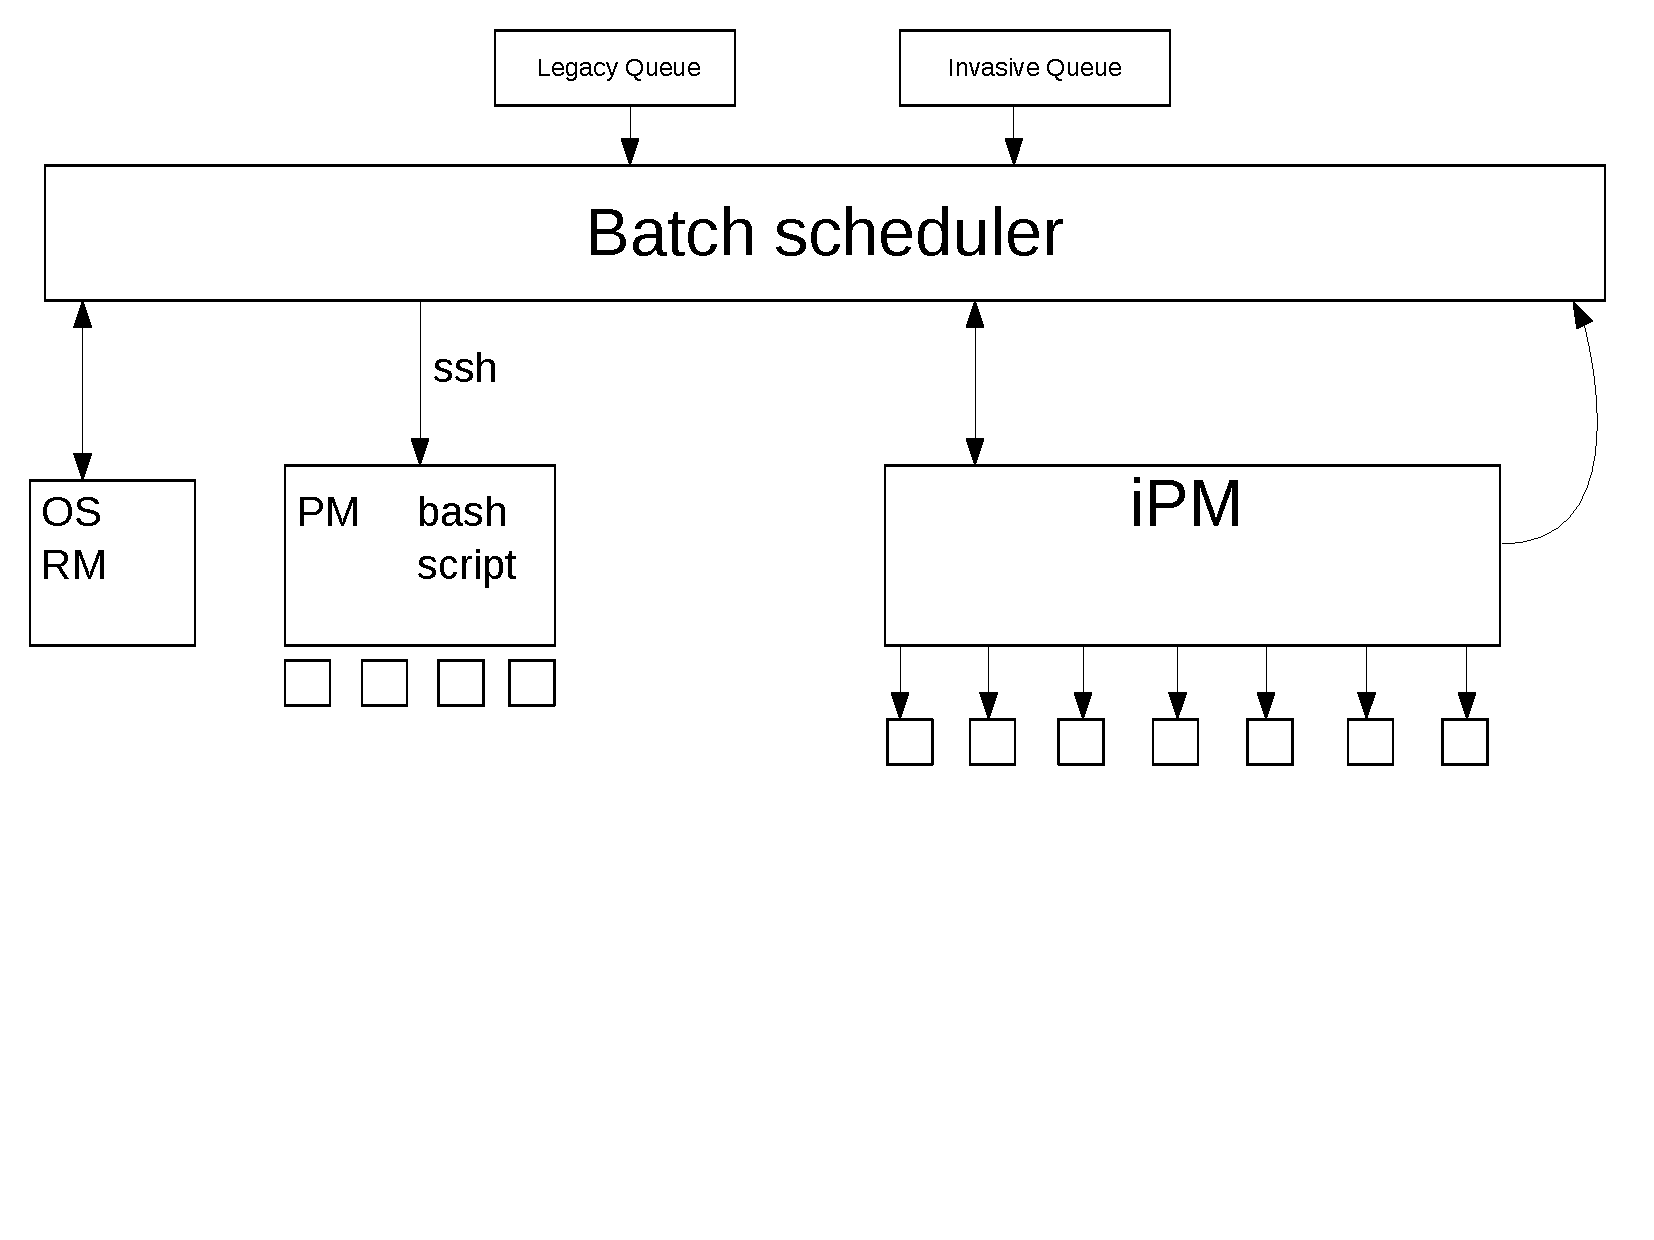
\includegraphics[width=0.65\textwidth, clip, trim=0mm 60mm 0mm 0mm]{data/architecture.pdf}
%\vspace{-0.15in}
%\caption{Invasive resource management architecture}
%\label{fig:arch}
%\end{figure}
\nocite{fontaine,gao,poorzahedy2,tianze,leblanc,kuo,poorzahedy1,wen}

\bibliographystyle{unsrt}
% Literature sources are to be found in seminarpaper.bib
\bibliography{nishanth}

\end{document}
